\section{Ablations}
\label{sec:ablations}

\paragraph{Experimental details.} We train transformers with positional embedding, pre-layer norm, $\softmax$ activation in \attn, and ReLU activation in \mlp. 
We use Adam with constant learning rate $0.0003$, $\beta_1=0.9$, $\beta_2=0.99$, $\eps=10^{-8}$, and a weight decay of $0.01$. We choose a learning rate of $0.03$ for the SGD. In each training step, we resample from the BB task with a batch size of $B=512$ and sequence length $N=256$. Unless otherwise specified, the model is trained for $10,000$ steps. Results are consistent across different random seeds.

\paragraph{More attention plots}: Figure \ref{appfigure:more-attn} presents more attention-weight heat maps of the one-layer transformer model trained on the BB task. All attention maps show the attention sink phenomenon. Interestingly, the trigger tokens serve as attention sinks in some inputs.
\begin{figure}[t]
  \centering
  \begin{minipage}{0.3\textwidth}
      \centering
      \subcaption{\small Sequence 0}
      \vspace{-.2em}
      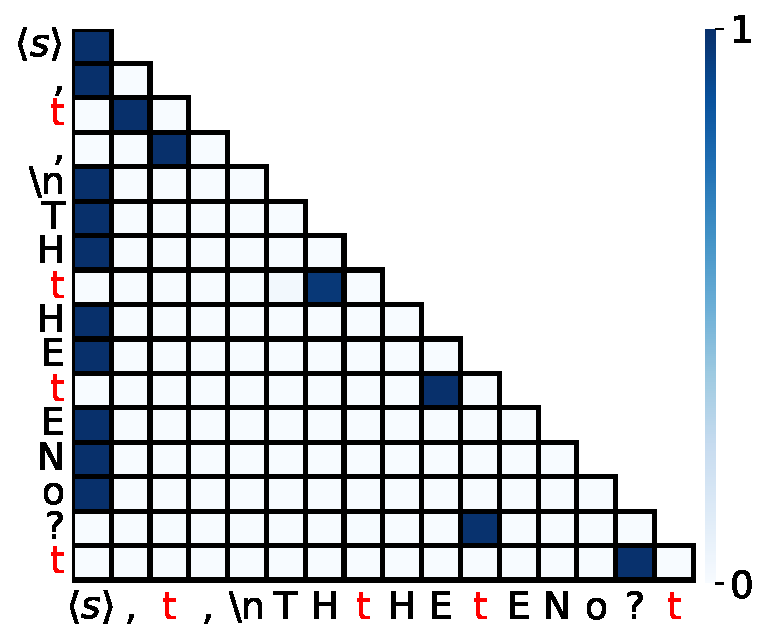
\includegraphics[width=\linewidth]{Figures/BBM_appendix/app_attn_fig1.pdf}
  \end{minipage}
  % \hspace{-1em}
  \begin{minipage}{0.3\textwidth}
      \centering
      \subcaption{\small Sequence 1}
      \vspace{-.2em}
      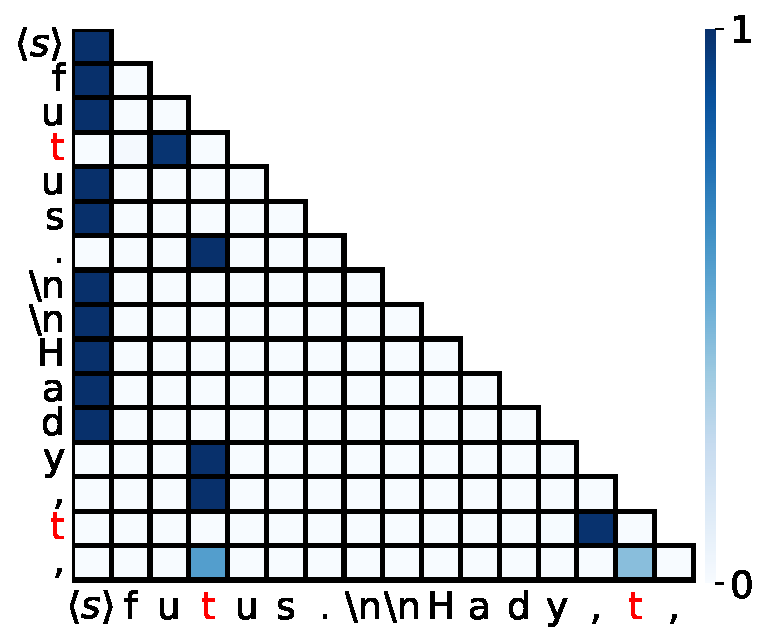
\includegraphics[width=\linewidth]{Figures/BBM_appendix/app_attn_fig2.pdf}
  \end{minipage}
  % \hspace{-1em}
  \begin{minipage}{0.3\textwidth}
      \centering
      \subcaption{\small Sequence 2}
      \vspace{-.2em}
      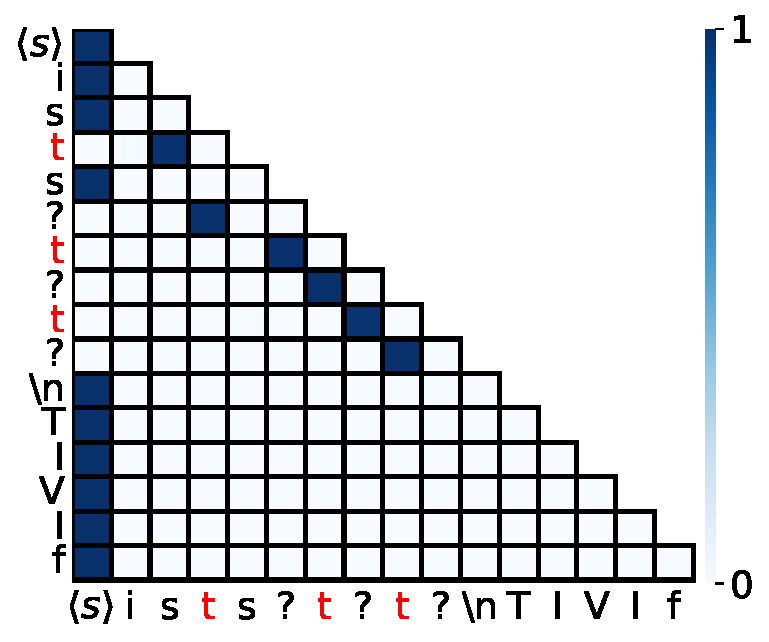
\includegraphics[width=\linewidth]{Figures/BBM_appendix/app_attn_fig3.pdf}
  \end{minipage}
  % \vspace{-1em}
  \caption{\small Attention plots of the one-layer transformer trained on the Bigram-Backcopy task.}
  \label{appfigure:more-attn}
  \vspace{-1em}
\end{figure}

\subsection{Ablations of different model structures trained on the Bigram-Backcopy task.}

\paragraph{Exploring the minimal structure for massive norms.} Figure \ref{appfigure:massive_minimal} presents the difference of residual norms between the \bos~token and others ($\|\res_{\bos}\|-\E_{\tok\neq\bos}[\|\res_{\tok}\|]$), with different combinations of model structures. The $3\times \TF$ and $2\times \TF+\mlp$ are two outliers, showing clear evidence of residual state peaks.

\begin{figure}
    \centering
    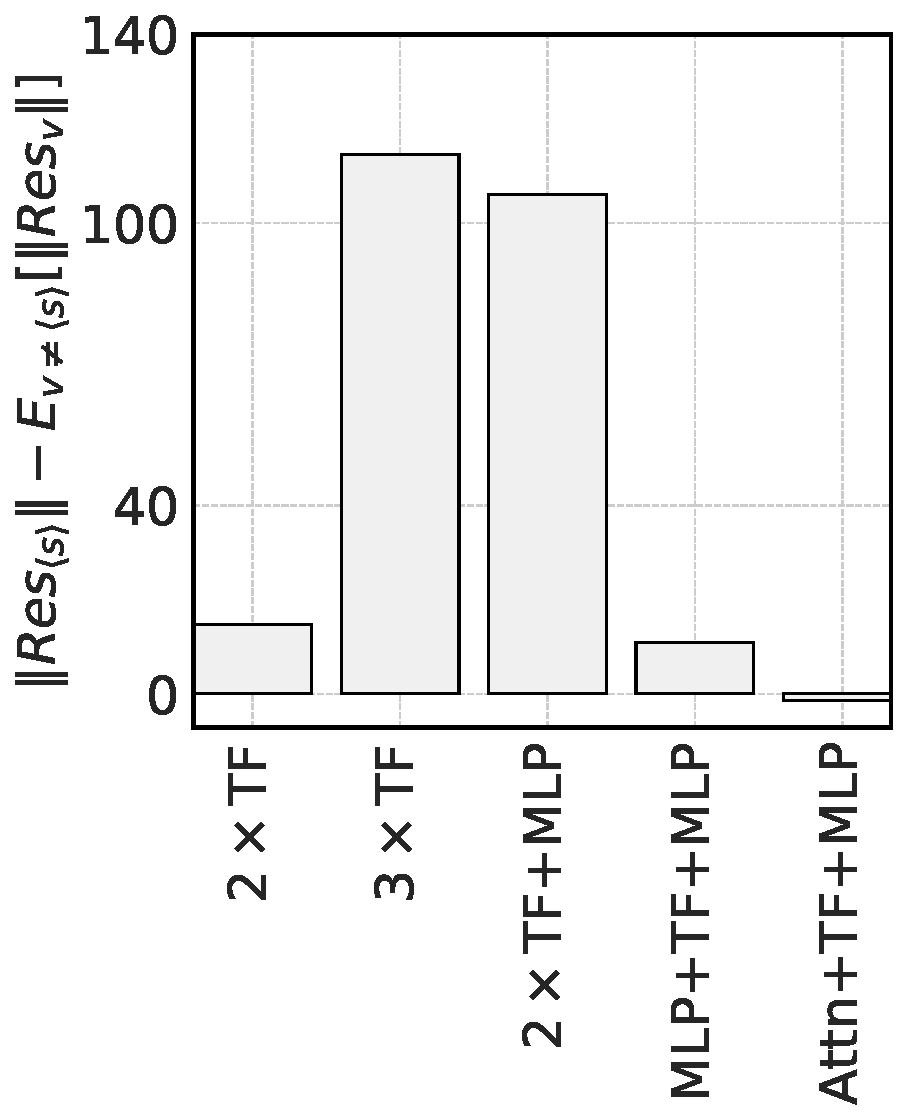
\includegraphics[width=0.7\linewidth]{Figures/BBM_appendix/massive_norm_minimal.pdf}
    \caption{\small Minimal structures to elicit residual state peaks. We use $A+B+C$ to indicate the model with structure $A$, $B$, $C$ in layers 0, 1, and 2, respectively.}
    \label{appfigure:massive_minimal}
\end{figure}

\paragraph{Attention plots, value state norms, and residual norms for a three-layer transformer trained on BB task.} Figures \ref{appfigure:massive-attn}, \ref{appfigure:massive-value-norm}, and \ref{appfigure:massive-norm} show the extreme token phenomena in a three-layer transformer. The residual state peaks show different phenomena from those in LLMs, with the last layer output increasing the residual norms of non-\bos~tokens. Figure \ref{figure:extreme-token}
 demonstrates that the residual state norms of \bos~drop match the magnitudes of other tokens at the last layer. 
\begin{figure}[t]
  \centering
  \begin{minipage}{0.3\textwidth}
      \centering
      \subcaption{\small Layer 0}
      \vspace{-.2em}
      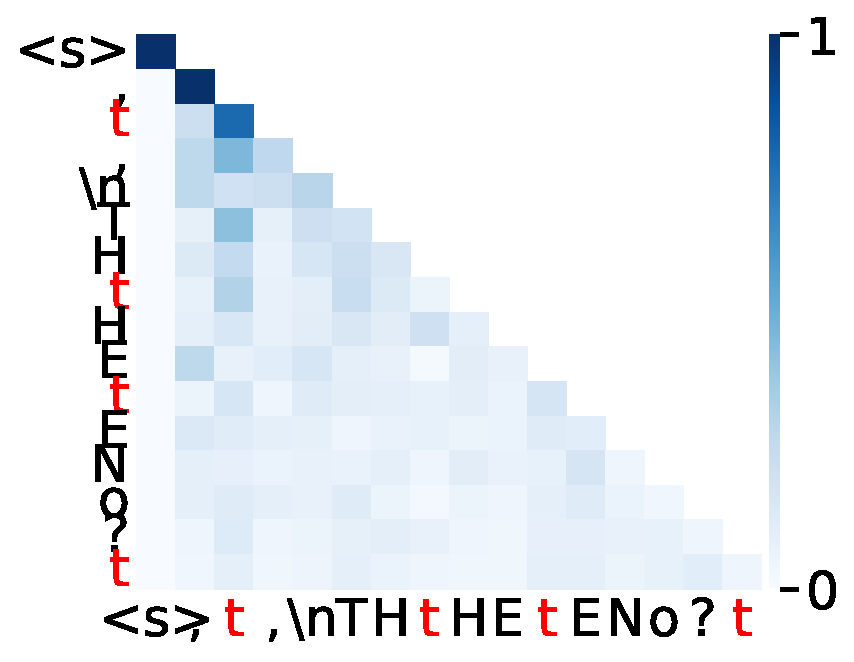
\includegraphics[width=\linewidth]{Figures/BBM_appendix/massive_attn_fig0.pdf}
  \end{minipage}
  % \hspace{-1em}
  \begin{minipage}{0.3\textwidth}
      \centering
      \subcaption{\small Layer 1}
      \vspace{-.2em}
      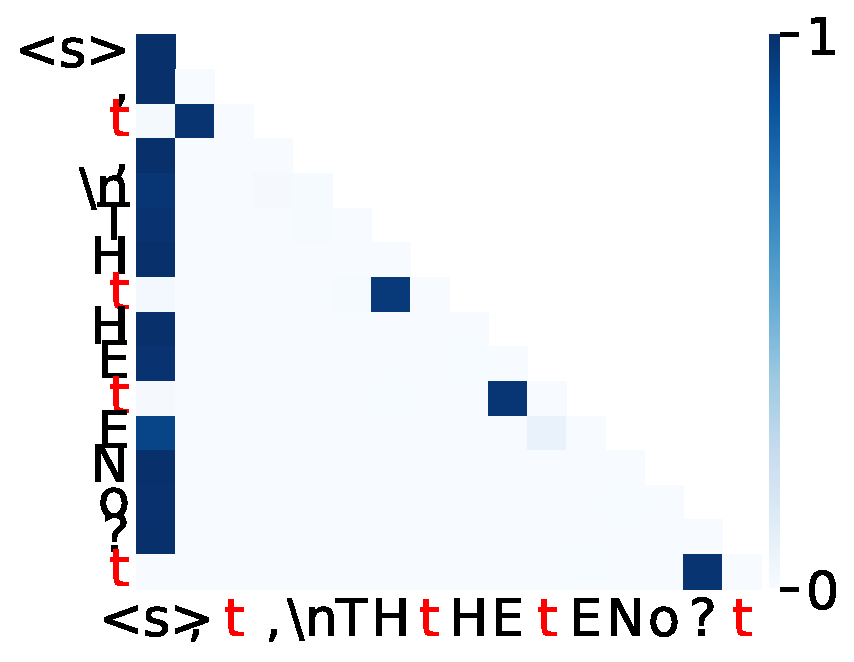
\includegraphics[width=\linewidth]{Figures/BBM_appendix/massive_attn_fig1.pdf}
  \end{minipage}
  % \hspace{-1em}
  \begin{minipage}{0.3\textwidth}
      \centering
      \subcaption{\small Layer 2}
      \vspace{-.2em}
      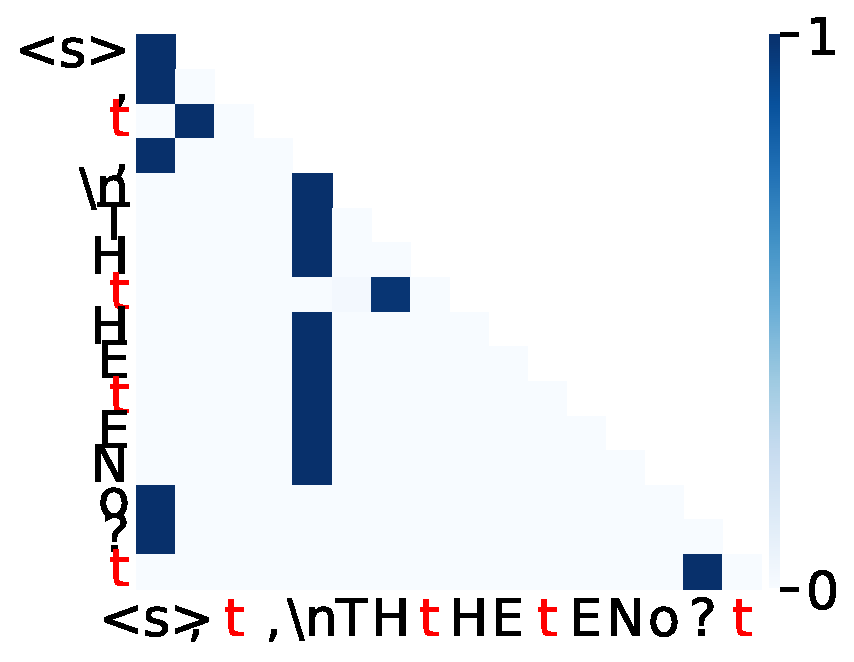
\includegraphics[width=\linewidth]{Figures/BBM_appendix/massive_attn_fig2.pdf}
  \end{minipage}
  % \vspace{-1em}
  \caption{\small Value state norms of three-layer transformer trained on the BB task}
  \label{appfigure:massive-attn}
  \vspace{-1em}
\end{figure}

\begin{figure}[t]
  \centering
  \begin{minipage}{0.3\textwidth}
      \centering
      \subcaption{\small Layer 0}
      \vspace{-.2em}
      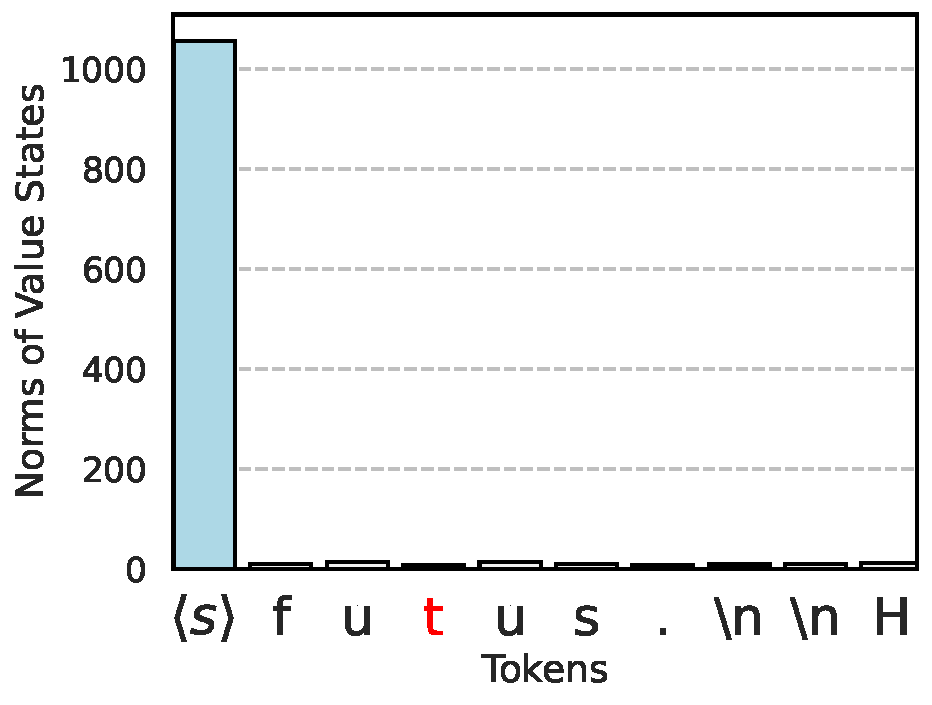
\includegraphics[width=\linewidth]{Figures/BBM_appendix/value_states_layer_0.pdf}
  \end{minipage}
  % \hspace{-1em}
  \begin{minipage}{0.3\textwidth}
      \centering
      \subcaption{\small Layer 1}
      \vspace{-.2em}
      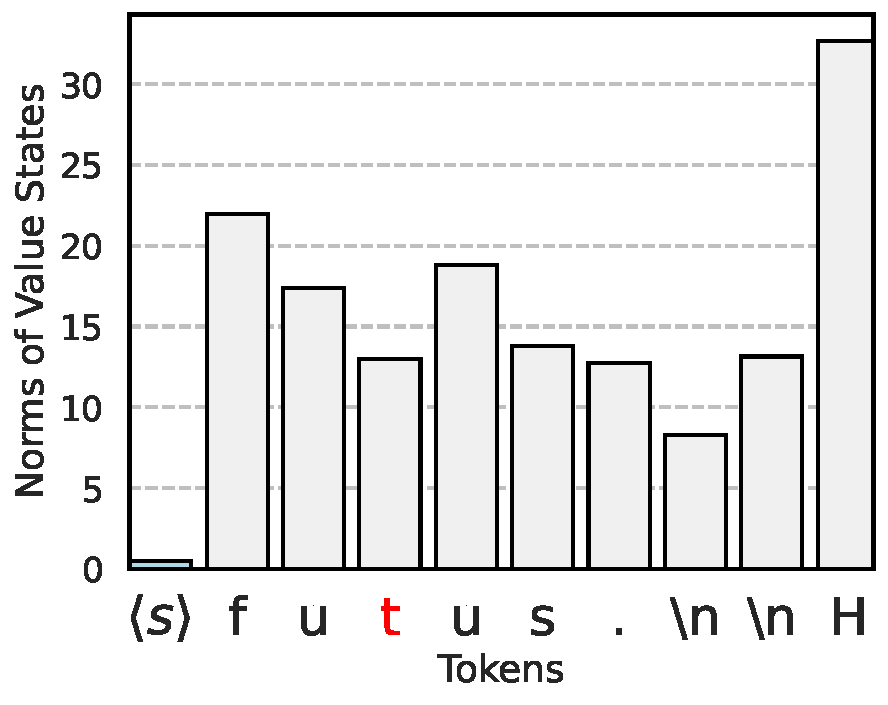
\includegraphics[width=\linewidth]{Figures/BBM_appendix/value_states_layer_1.pdf}
  \end{minipage}
  % \hspace{-1em}
  \begin{minipage}{0.3\textwidth}
      \centering
      \subcaption{\small Layer 2}
      \vspace{-.2em}
      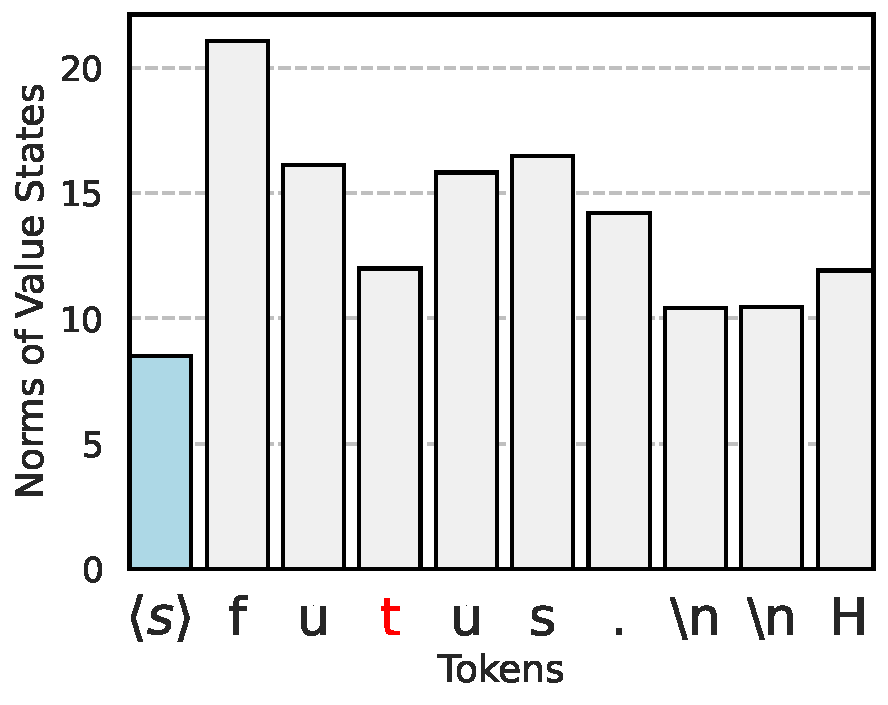
\includegraphics[width=\linewidth]{Figures/BBM_appendix/value_states_layer_2.pdf}
  \end{minipage}
  % \vspace{-1em}
  \caption{\small Value state norms of three-layer transformer trained on the BB task}
  \label{appfigure:massive-value-norm}
  \vspace{-1em}
\end{figure}


\begin{figure}[t]
  \centering
  \begin{minipage}{0.3\textwidth}
      \centering
      \subcaption{\small Layer 0}
      \vspace{-.2em}
      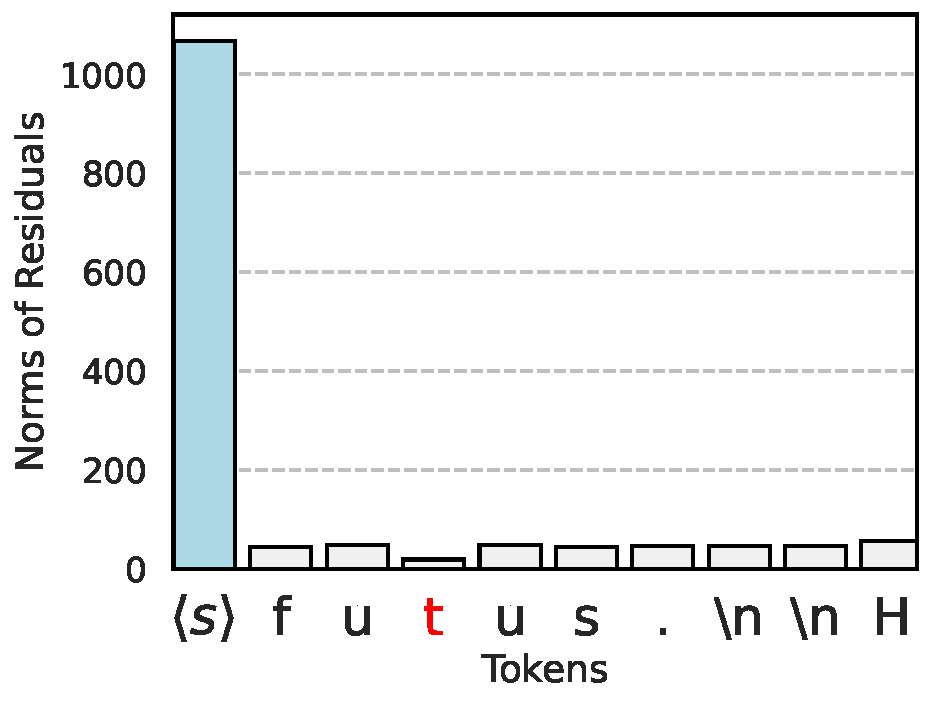
\includegraphics[width=\linewidth]{Figures/BBM_appendix/norms_layer_0.pdf}
  \end{minipage}
  % \hspace{-1em}
  \begin{minipage}{0.3\textwidth}
      \centering
      \subcaption{\small Layer 1}
      \vspace{-.2em}
      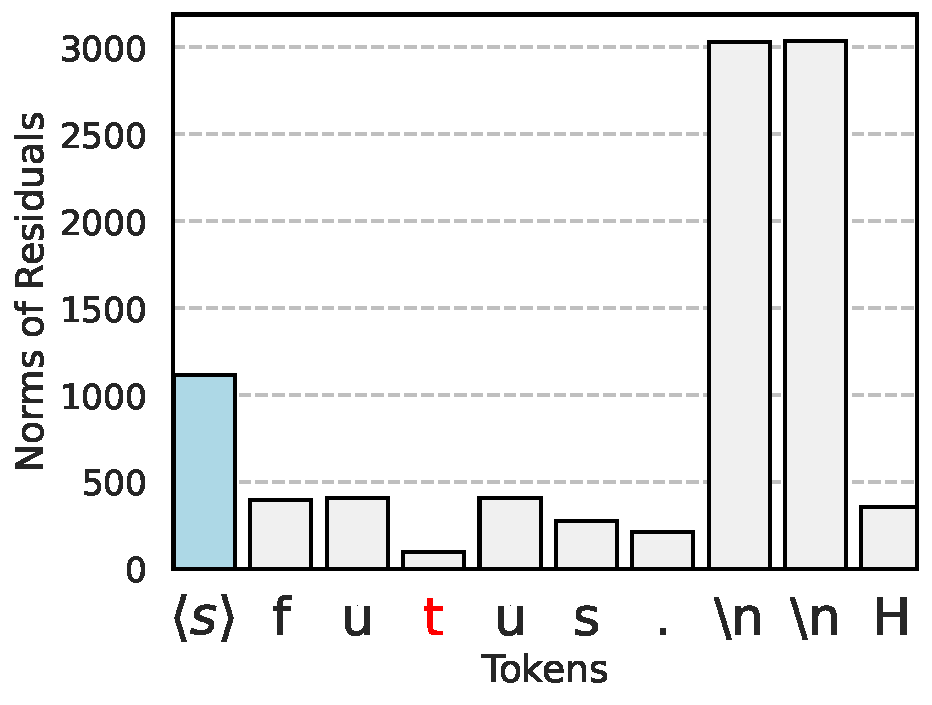
\includegraphics[width=\linewidth]{Figures/BBM_appendix/norms_layer_1.pdf}
  \end{minipage}
  % \hspace{-1em}
  \begin{minipage}{0.3\textwidth}
      \centering
      \subcaption{\small Layer 2}
      \vspace{-.2em}
      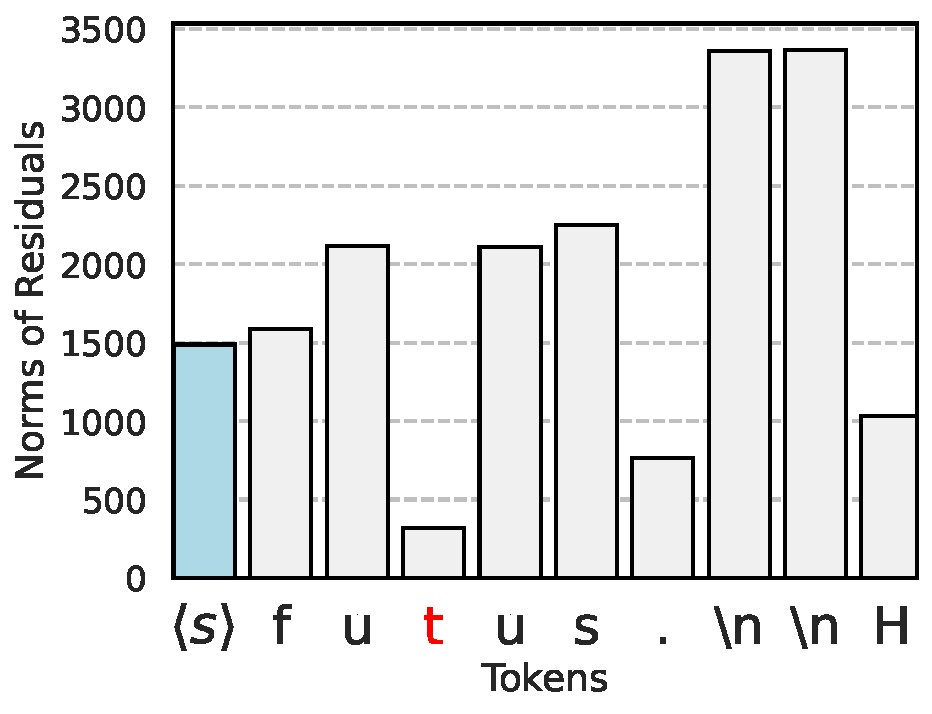
\includegraphics[width=\linewidth]{Figures/BBM_appendix/norms_layer_2.pdf}
  \end{minipage}
  % \vspace{-1em}
  \caption{\small Residual state norms of three-layer transformer trained on the BB task}
  \label{appfigure:massive-norm}
  \vspace{-1em}
\end{figure}

% \paragraph{Exploring the minimal structure for massive norms.} Figure \ref{appfigure:massive_minimal} presents the difference of residual norms between the \bos~token and others ($\|\res_{\bos}\|-\E_{\tok\neq\bos}[\|\res_{\tok}\|]$), with different combinations of model structures. The $3\times \TF$ and $2\times \TF+\mlp$ are two outliers, showing clear evidence of residual state peaks.
\paragraph{Statics and dynamics of the simplified model in Theorem \ref{thm:main}.} With the simplified model structure in Figure \ref{figure:simple-model}, we pre-train the model using Adam with learning rate $0.03$. Figure \ref{appfigure:simple-static} and \ref{appfigure:simple-dynamic} show results that match both the theory and the observations of the one-layer transformer. 

\begin{figure}[t]
  \centering
  \begin{minipage}{0.3\textwidth}
      \centering
      \subcaption{\small Attention weights}
      \vspace{-.2em}
      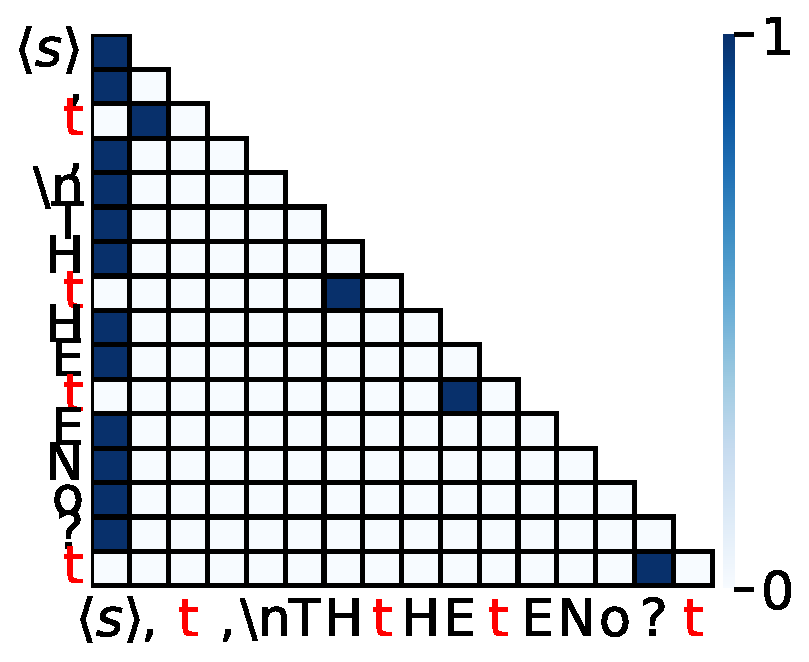
\includegraphics[width=\linewidth]{Figures/BBM_appendix/simple_attn_fig0.pdf}
  \end{minipage}
  % \hspace{-1em}
  \begin{minipage}{0.3\textwidth}
      \centering
      \subcaption{\small Value state norms}
      \vspace{-.2em}
      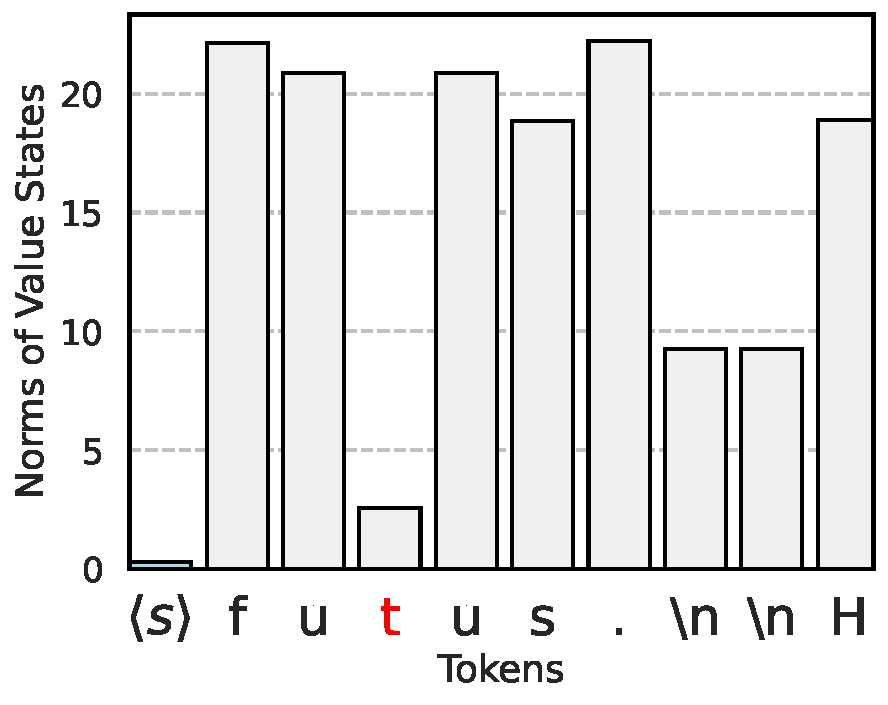
\includegraphics[width=\linewidth]{Figures/BBM_appendix/simple_value_states_layer_0.pdf}
  \end{minipage}
  \caption{\small The simplified model structure trained on the BB task.}
  \label{appfigure:simple-static}
  \vspace{-1em}
\end{figure}

\begin{figure}[t]
  \centering
  \begin{minipage}{0.3\textwidth}
      \centering
      \subcaption{\small First 1000 steps}
      \vspace{-.2em}
      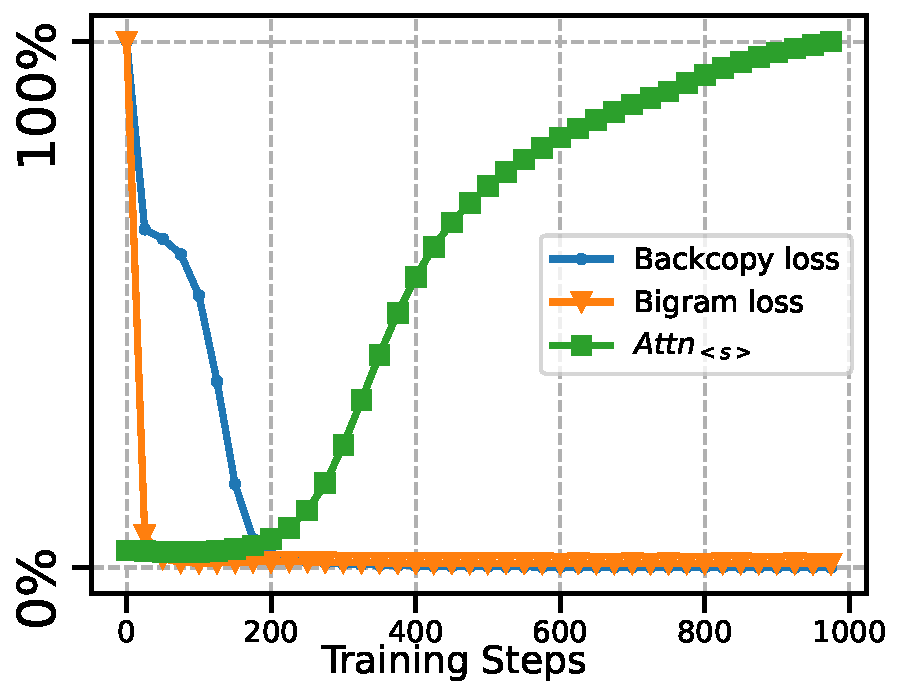
\includegraphics[width=\linewidth]{Figures/BBM_appendix/simple_dynamics.pdf}
  \end{minipage}
  % \hspace{-1em}
  \begin{minipage}{0.3\textwidth}
      \centering
      \subcaption{\small From 0 to 10000 steps}
      \vspace{-.2em}
      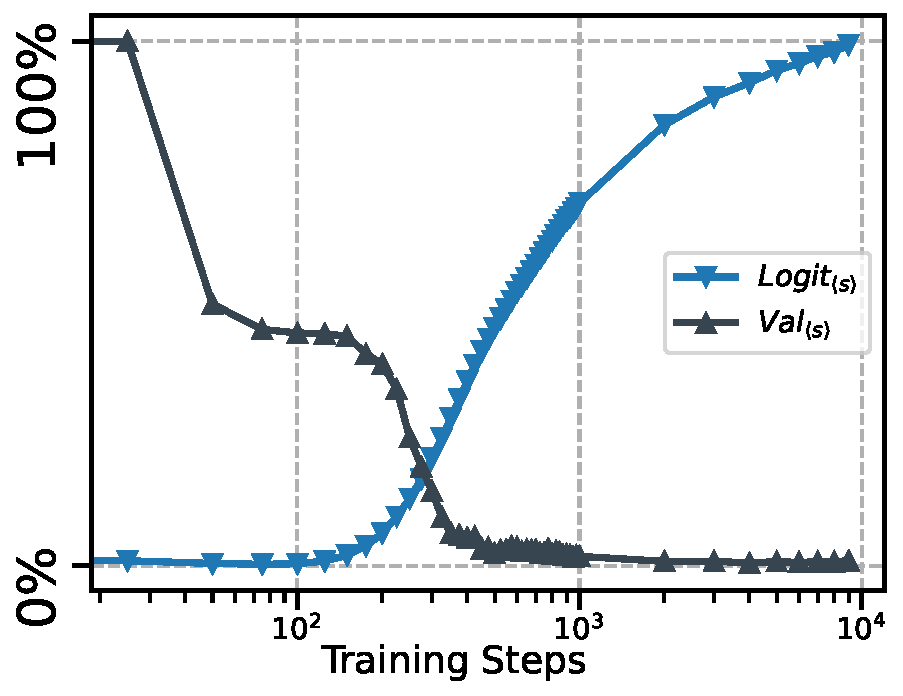
\includegraphics[width=\linewidth]{Figures/BBM_appendix/simple_dynamics_logit.pdf}
  \end{minipage}
  \caption{\small The dynamics of the simplified model structure trained on the BB task. \textit{Left (a):} The training curves match the one-layer transformer. \textit{Right (b):} The logit curve is close to the logarithmic growth predicted in Theorem \ref{thm:main}.}
  \label{appfigure:simple-dynamic}
  \vspace{-1em}
\end{figure}

\subsection{Variations of the Bigram-Backcopy task}

\paragraph{Bigram-Backcopy task without the \bos~token.} We train a one-layer transformer on the BB task without the \bos~token. Figure \ref{appfigure:no-bos-extreme} shows that the \bos~token is perhaps not the extreme token. Instead, trigger tokens and delimiter tokens seem to become extreme tokens. The results indicate that initial tokens may not be the only candidates for the extreme token, partially explaining why delimiter tokens could also be extreme tokens in LLMs.
\begin{figure}[t]
  \centering
  \begin{minipage}{0.35\textwidth}
      \centering
      \subcaption{\small Attention weights}
      \vspace{-.2em}
      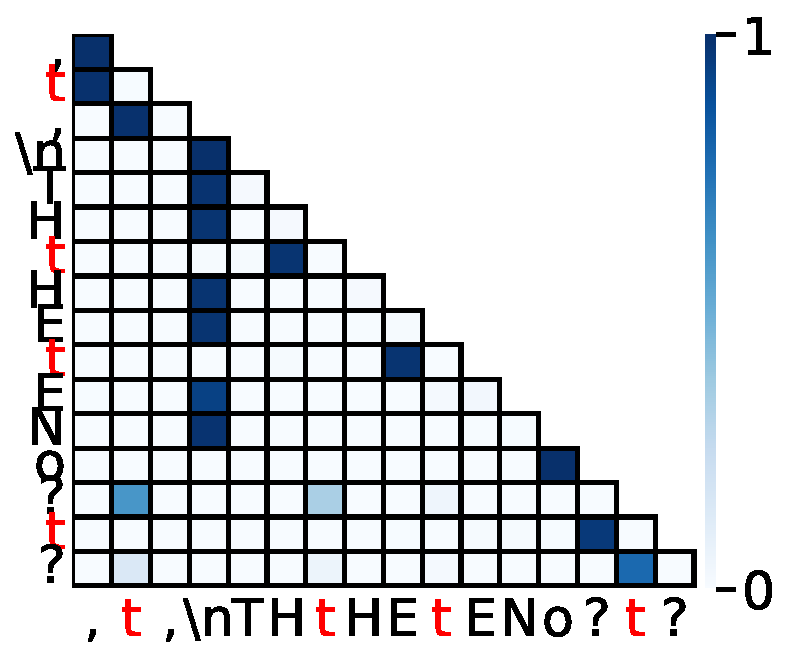
\includegraphics[width=\linewidth]{Figures/BBM_appendix/no_bos_attn_fig0.pdf}
  \end{minipage}
  \begin{minipage}{0.35\textwidth}
      \centering
      \subcaption{\small Value state norms}
      \vspace{-.2em}
      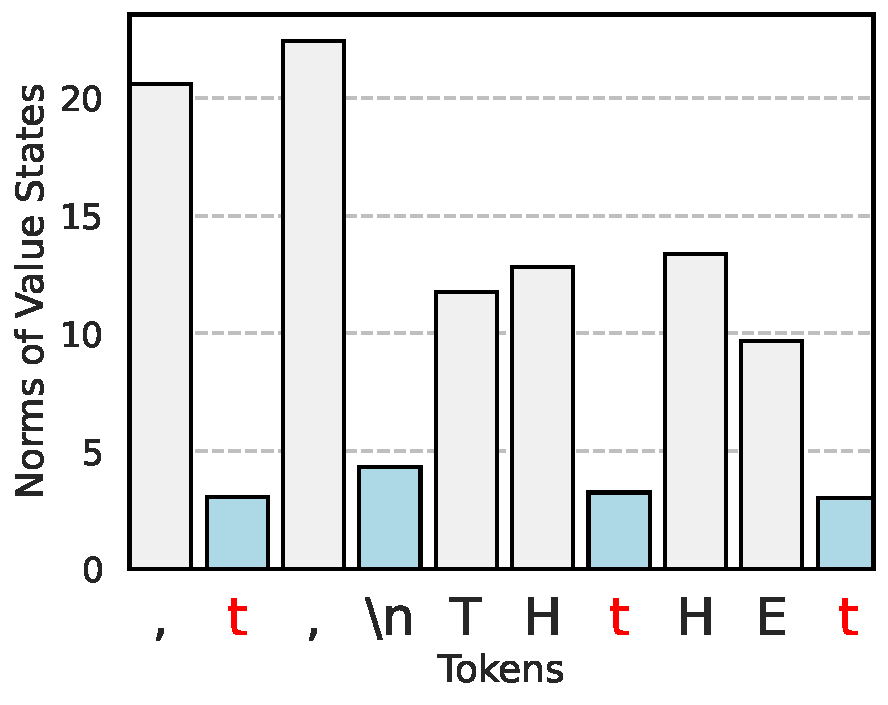
\includegraphics[width=\linewidth]{Figures/BBM_appendix/no_bos_value_states_layer_0.pdf}
  \end{minipage}
  % \vspace{-1em}
\caption{\small Attention weights and value state norms of a one-layer transformer trained on the BB task without the \bos~token.}
  \label{appfigure:no-bos-extreme}
  \vspace{-1em}
\end{figure}


\paragraph{The Bigram-Skip-one (BS) task.} We make slight modifications to the Bigram-Backcopy task. On trigger tokens, instead of copying the preceding token, we sample from the bigram-probability of the preceding token $\texttt{P}(\cdot\mid \text{Second-to-last token})$. We train a one-layer transformer on it using the same configuration as the BB task. Figure \ref{appfigure:BS-findings} shows that extreme token phenomena are mitigated. The reason is that trained under BS, both the value states $\vall_\tok$ and the token embedding $\embd_\tok$ give the logit of the bigram transition probability. Therefore, other than having attention sink on the \bos~token, self-attention becomes a new possibility to achieve the active-dormant mechanism.

\begin{figure}[t]
  \centering
  \begin{minipage}{0.38\textwidth}
      \centering
      \subcaption{\small The Bigram-Skip-one task}
      % \label{fig:bbm-dgp}
      \vspace{-.2em}
      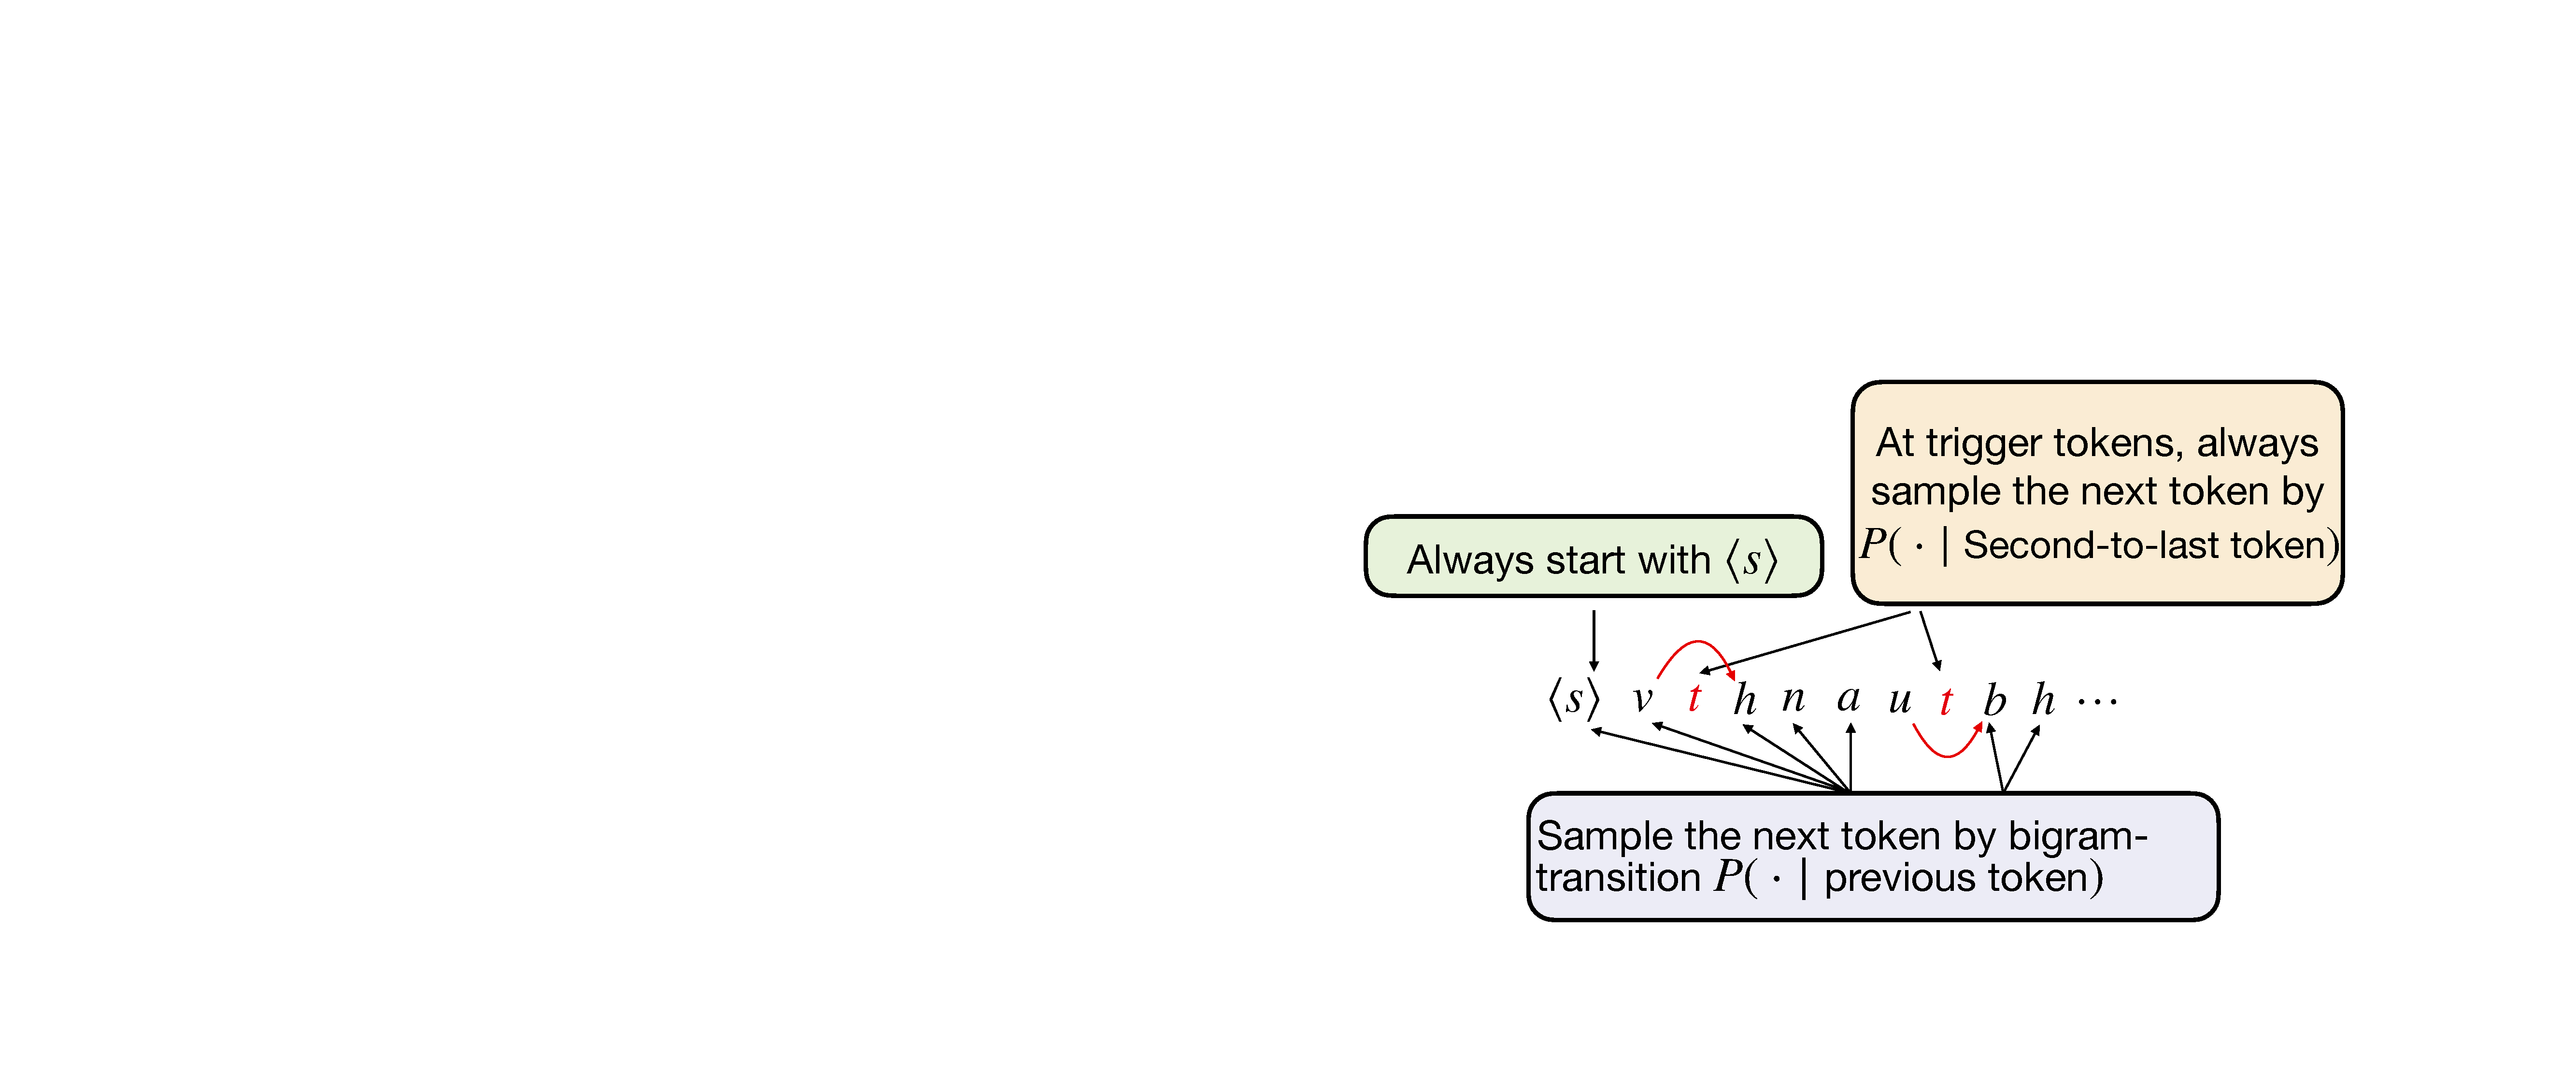
\includegraphics[width=\linewidth]{Figures/BBM_appendix/BS.pdf}
  \end{minipage}
  % \hspace{-1em}
  \begin{minipage}{0.26\textwidth}
      \centering
      \subcaption{\small Attention pattern}
      % \label{fig:bbm-attn}
      \vspace{-.2em}
      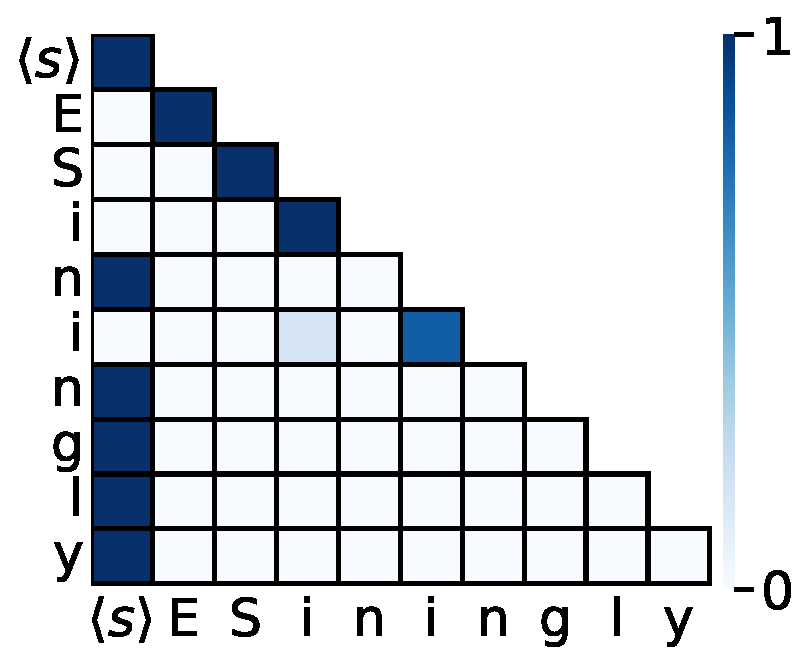
\includegraphics[width=\linewidth]{Figures/BBM_appendix/BS_attn.pdf}
  \end{minipage}
  % \hspace{-1em}
  \begin{minipage}{0.27\textwidth}
      \centering
      \subcaption{\small Small value states}
      \vspace{0pt}
      % \label{fig:bbm-value}
      \vspace{-.2em}
      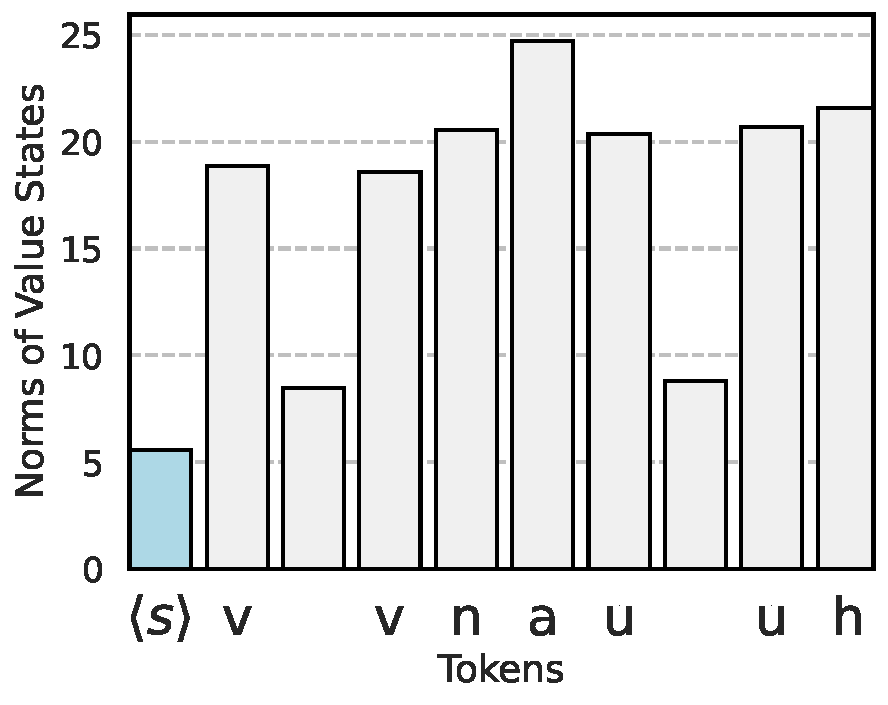
\includegraphics[width=\linewidth]{Figures/BBM_appendix/BS_value.pdf}
  \end{minipage}
  % \vspace{-1em}
  \caption{\small \textbf{Experiments on the Bigram-Skip-one task.} 
  All phenomena are close to those in the BB task, but with diagonal attention sinks and relatively larger $\|\vall_\bos\|$ compared with Figure \ref{figure:pretraining-findings}.}
  \label{appfigure:BS-findings}
  \vspace{-1em}
\end{figure}


